
%%%% First frame: beschreibung der Ansätze, um Sentiment-Werte zu bestimmen.
% Im Quellcode werden durch den \alt Befehl jeweils die Box hervorgehoben, auf die sich der Text unten bezieht.
\begin{frame}
\frametitle{Module - Sentiment - Ansätze}

\begin{columns}[c]

  \begin{column}{0.33\textwidth}
  \begin{center}
     \alt<2,3>{
    \begin{tikzpicture}
 %  \draw (0,0) rectangle (4,2);
%  \draw [rounded corners=5pt] (0,0) -- (0,2) -- (4,2) -- (4,0) -- (0,0);
  \node [thick, draw = black, rounded corners, text width = 3cm] { 
 	 \begin{tabular}{c} 
 	 	Emoticon-Liste \\ 
 	 	\\
  		\includegraphics[width=.72\textwidth]{../img/smiley_4.pdf}
 	\end{tabular} 
	};
    \end{tikzpicture} 
    }
    {
      \begin{tikzpicture}
 %  \draw (0,0) rectangle (4,2);
%  \draw [rounded corners=5pt] (0,0) -- (0,2) -- (4,2) -- (4,0) -- (0,0);
  \node [ultra thick, draw = black, rounded corners, text width = 3cm] { 
 	 \begin{tabular}{c} 
 	 	Emoticon-Liste \\ 
 	 	\\
  		\includegraphics[width=.72\textwidth]{../img/smiley_4.pdf}
 	\end{tabular} 
	};
    \end{tikzpicture}   
    }
 %   MAE: 0.8
      \end{center}
  \end{column}

  \begin{column}{0.33\textwidth}
  \begin{center}
   \alt<1,3>{
    \begin{tikzpicture}
 %  \draw (0,0) rectangle (4,2);
%  \draw [rounded corners=5pt] (0,0) -- (0,2) -- (4,2) -- (4,0) -- (0,0);
  \node [thick, draw = black, rounded corners] { 
 	 \begin{tabular}{c} 
 	 	\hphantom{aa}Wörterbuch\hphantom{aa}  \\ 
 	 	\\
  		\includegraphics[width=.31\textwidth]{../img/registry-book.pdf}
 	\end{tabular} 
	};
    \end{tikzpicture} 
    }
    {
    \begin{tikzpicture}
 %  \draw (0,0) rectangle (4,2);
%  \draw [rounded corners=5pt] (0,0) -- (0,2) -- (4,2) -- (4,0) -- (0,0);
  \node [ultra thick, draw = black, rounded corners] { 
 	 \begin{tabular}{c} 
 	 	\hphantom{aa}Wörterbuch\hphantom{aa}  \\ 
 	 	\\
  		\includegraphics[width=.31\textwidth]{../img/registry-book.pdf}
 	\end{tabular} 
	};
    \end{tikzpicture}     
    }
%     MAE: 0.8
      \end{center}
  \end{column}
 
  \begin{column}{0.33\textwidth}
  \begin{center}
   \alt<1,2>{
    \begin{tikzpicture}
 %  \draw (0,0) rectangle (4,2);
%  \draw [rounded corners=5pt] (0,0) -- (0,2) -- (4,2) -- (4,0) -- (0,0);
  \node [thick, draw = black, rounded corners] { 
 	 \begin{tabular}{c} 
 	 	Machine  \\ 
 	 	\hphantom{aaa}Learning\hphantom{aaa} \\
  		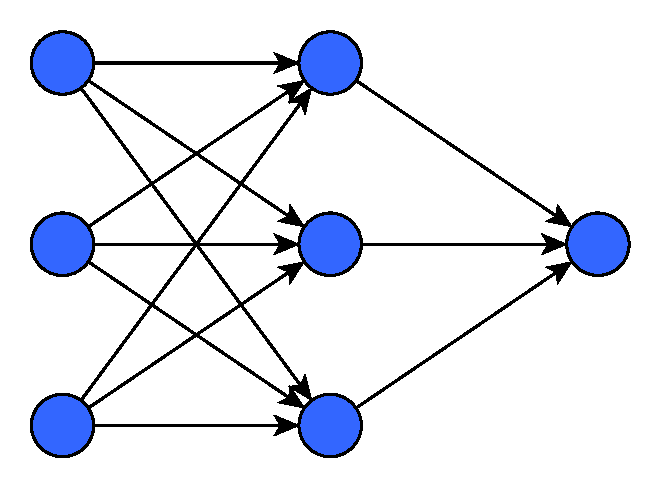
\includegraphics[width=.4\textwidth]{../img/neuralNetwork.pdf}
 	\end{tabular} 
	};
    \end{tikzpicture} 
    }
	{
	\begin{tikzpicture}
 %  \draw (0,0) rectangle (4,2);
%  \draw [rounded corners=5pt] (0,0) -- (0,2) -- (4,2) -- (4,0) -- (0,0);
  \node [ultra thick, draw = black, rounded corners] { 
 	 \begin{tabular}{c} 
 	 	Machine  \\ 
 	 	\hphantom{aaa}Learning\hphantom{aaa} \\
  		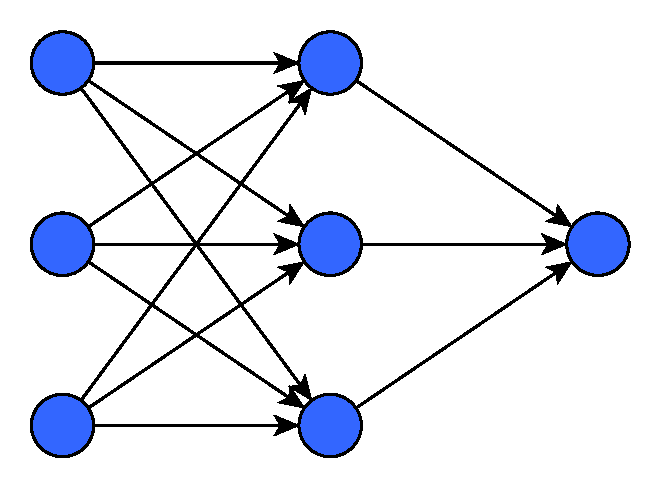
\includegraphics[width=.4\textwidth]{../img/neuralNetwork.pdf}
 	\end{tabular} 
	};
    \end{tikzpicture} 
	}    
 %    MAE: 0.4
      \end{center}
  \end{column}
  
\end{columns}

%\begin{columns}[t]
%\column{.3\textwidth}
%\begin{block}{Emoticon-Liste}
%\centering
%\includegraphics[width=.31\textwidth]{../img/registry-book.pdf}
%\end{block}
%\column{.3\textwidth}
%\begin{block}{Wörterbuch}
%\centering
%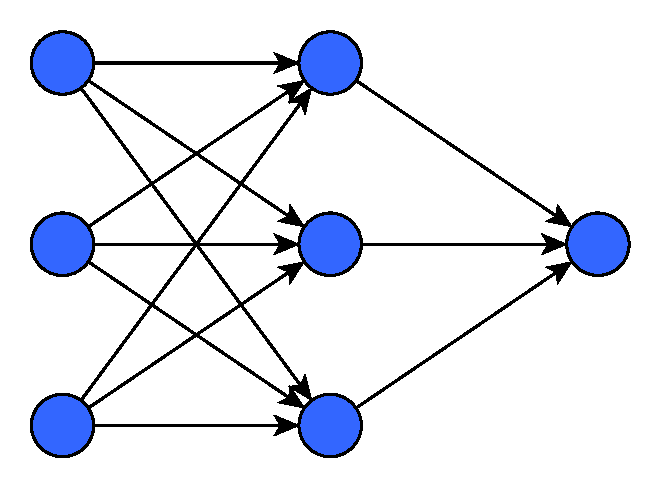
\includegraphics[width=.4\textwidth]{../img/neuralNetwork.pdf}
%\end{block}
%\column{.3\textwidth}
%\begin{block}{Machine Learning}
%\centering
%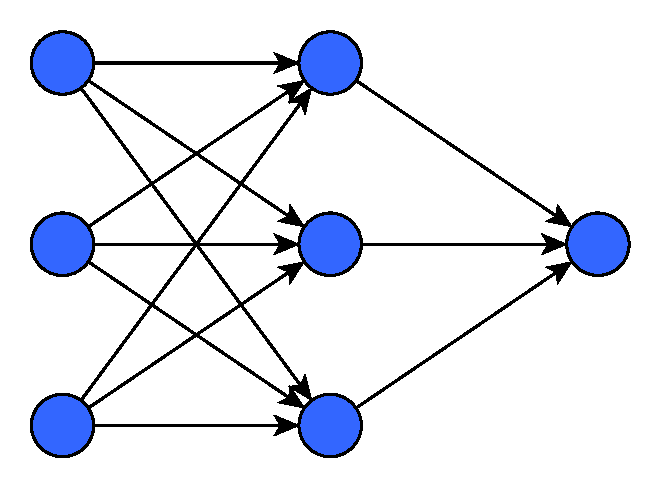
\includegraphics[width=.4\textwidth]{../img/neuralNetwork.pdf}
%\end{block}
%\end{columns}

\bigskip

\begin{itemize}
\item<1-> I love puppies \alt<1>{\color{SentiGreen}\textbf{:-)} }{:-)}
%
\item<2-3> I \alt<2>{\textcolor{SentiGreen}{\textbf{love}}}{love} puppies :-)
%
\item<3>  
\alt<3>{\textcolor{SentiLightRed}{\textbf{I}}}{I} 
\alt<3>{\textcolor{SentiGreen}{\textbf{love}}}{love} 
\alt<3>{\textcolor{SentiDarkGreen}{\textbf{puppies}}}{puppies} 
\alt<3>{\textcolor{SentiGreen}{\textbf{:-)}}}{:-)} 
%
\end{itemize}

\bigskip

\end{frame}

%%%%%%%%%%%%%%%%%%%%%%%%%%%%%%%%%%%%%%%%%%%%%%%%%%%%%
%%%%%%%%%%%%%%%%%%%%%%%%%%%%%%%%%%%%%%%%%%%%%%%%%%%%%
%%%%%%%%%%%%%%%%%%%%%%%%%%%%%%%%%%%%%%%%%%%%%%%%%%%%%
%%%%%%%%%%%%%%%%%%%%%%%%%%%%%%%%%%%%%%%%%%%%%%%%%%%%%

\begin{frame}{Module - Sentiment - Machine\,Learning\,mit\,Regression}

\begin{itemize}

\item Trainingsdaten:
\begin{itemize}
\item ``I love puppies''
\item ``I hate puppies''
%\item Sätze:
%\begin{itemize}
%\item I love puppies
%\item I hate puppies
%\end{itemize}

\pause

\item Merkmalsmatrix:
\item[]
\begin{tabular}{cccc|c}
I & love & hate & puppies & Sentiment \\
1 & 1 & 0 & 1 & \textcolor{SentiGreen}{\(+1\)} \\
1 & 0 & 1 & 1 & \textcolor{red}{\(-1\)} \\
\end{tabular}
\end{itemize}

\pause

\item Regressionsmodell:
\item[]
\begin{tabular}{cccc}
I & \textcolor{SentiGreen}{love} & \textcolor{red}{hate} & puppies \\
0 & \textcolor{SentiGreen}{\(+1\)} & \textcolor{red}{\(-1\)} & 0 \\
\end{tabular}

\pause

\item Neue Tweets: z. B. ``I love kitties''
\item[]
\begin{tabular}{ccccc}
I & & \alt<5>{\textcolor{SentiGreen}{love}}{love} & kitties & \\

\pause

0 & + & \textcolor{SentiGreen}{1} &  & \textcolor{SentiGreen}{\(=1\)} \\
\end{tabular}

\end{itemize}

\end{frame}

%%%%%%%%%%%%%%%%%%%%%%%%%%%%%%%%%%%%%%%%%%%%%%%%%%%%%
%%%%%%%%%%%%%%%%%%%%%%%%%%%%%%%%%%%%%%%%%%%%%%%%%%%%%
%%%%%%%%%%%%%%%%%%%%%%%%%%%%%%%%%%%%%%%%%%%%%%%%%%%%%
%%%%%%%%%%%%%%%%%%%%%%%%%%%%%%%%%%%%%%%%%%%%%%%%%%%%%

\begin{frame}{Module - Sentiment - Architektur}

\begin{figure}[p]
\centering
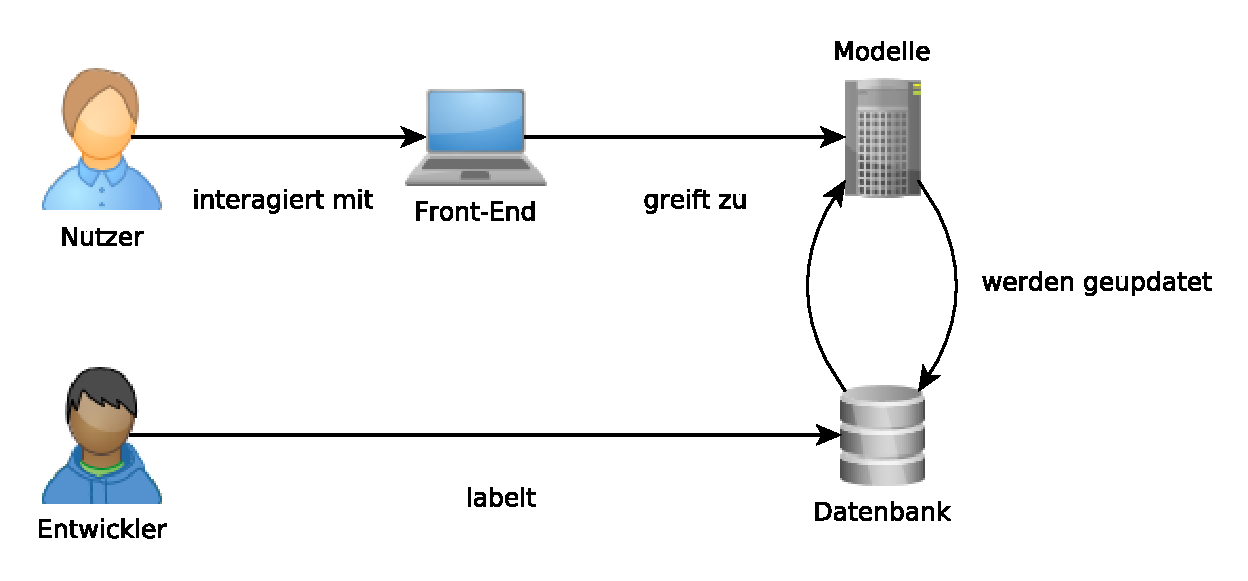
\includegraphics[scale=0.5]{../img/sentiment-architektur.pdf}
\end{figure}
\end{frame}

% Folie 4/4: Beschreiben, wie Sentiment-Werte dem Nutzer im Frontend dargestellt werden und wie Nutzer explorativ herausfinden kann, wie Wert zustande gekommen ist.
%%%%%%%%%%%%%%%%%%%%%%%%%%%%%%%%%%%%%%%%%%%%%%%%%%%%%
%%%%%%%%%%%%%%%%%%%%%%%%%%%%%%%%%%%%%%%%%%%%%%%%%%%%%
%%%%%%%%%%%%%%%%%%%%%%%%%%%%%%%%%%%%%%%%%%%%%%%%%%%%%
%%%%%%%%%%%%%%%%%%%%%%%%%%%%%%%%%%%%%%%%%%%%%%%%%%%%%

% \begin{frame}
% \frametitle{Module - Sentiment - Anzeige im Frontend}
% 
% 
% \begin{columns}
% \begin{column}{.49\textwidth}
% \begin{itemize}
% \item Diagramme mit Sentiment-Verteilung
% \item Filtern der Tweets nach Sentiment
% \item Einflussfaktoren auf Sentiment
% \item Trainingsdaten zu Einflussfaktoren
% \end{itemize}
%  \end{column}
% 
%  \begin{column}{.49\textwidth}
% \centering
% \includegraphics[height=.65\textheight]{../img/sentiment-overview1.png}
% % \\
% %\includegraphics[height=.49\textheight]{../img/sentiment-overview1.png}
%  \end{column}
% 
% \end{columns}
% 
% \end{frame}